\documentclass[a4paper, 12pt]{article}

\input{preamble}

\begin{document}
% This sets the default language for the listings package.
\lstset{language=Python}
\title{
\sffamily
\vspace{-1.7cm}
{\huge\textbf{Project 3 -- A Galton Board on a Rocking Ship}} \\[-0.4cm]
}
\author{
    \vspace{-0.4cm}
    \begin{minipage}[t]{0.45\textwidth}
\centering
Linus Brink\\
\href{mailto:brinkl@chalmers.se}{brinkl@chalmers.se}
\end{minipage}%
\hfill
\begin{minipage}[t]{0.45\textwidth}
\centering
Oscar Stommendal\\
\href{mailto:oscarsto@chalmers.se}{oscarsto@chalmers.se}
\vspace{0.5cm}
\end{minipage}
}
\date{\today}
\maketitle
\vspace{-1.5cm}
\section{Introduction}
In 1894, Sir Francis Galton introduced the Galton board -- a device that allows beads to fall through a series of pins, resulting in a binomial distribution of beads in the bottom compartments \cite{Galton1894NaturalInheritance}. However, if the number of rows and beads is sufficiently large, the distribution approaches a normal distribution, and the board thus serves as a physical demonstration of the Central Limit Theorem. About 50 years later, Alan Turing presented his paper ``Computing Machinery and Intelligence'', where he addressed the question ``\textit{Can machines think?}'' -- often considered as the birth of artificial intelligence \cite{IBMHistoryAI}. Today, of course, AI is a thriving field of research, with applications in a wide range of areas. The Galton board on the other hand, has not seen as much development since its inception. In this project however, we will explore a variant of the Galton board, where the board is placed on a rocking ship. This introduces an additional layer of complexity to the problem, as the rocking motion of the ship affects the trajectory of the beads as they fall through the pins. Using Approximate Bayesian Computation (ABC) and machine learning, we will attempt to infer the parameters governing the rocking motion of the ship based on observed data from the rocking Galton board.

\section{Theoretical Model}
In this project we consider a Galton board with $31$ rows of pegs, and hence $32$ compartments at the bottom. The beads are known to have a special kind of inertia, described by the hypothesis that a bead falling to the right/left at a peg will begin to spin clockwise/counter-clockwise. This spin will affect the trajectory of the bead at the next peg, making it more likely to fall in the same direction as before. The strength of this effect is governed by the bias parameter $\alpha$. Furthermore, we assume that earlier moves (more than one peg earlier) have no effect on the current move, and that the bias is zero at the first peg. The main goal of the project is to infer $\alpha$ from a series of observations of the final distribution of beads in the bottom compartments. However, since the board is placed on a rocking ship, there is an additional latent variable $s$ that affects the trajectory of the beads. This represents the current tilt of the ship, and varies uncontrollably from experiment to experiment. According to this model, the probability of a bead falling to the right (left) at a peg $P_+$ ($P_-$) is given by
\begin{equation}
    P_\pm = 0.5 \pm (\alpha M + s)\,,
\end{equation}
where $M = 0$ at the first peg, and $M = \pm 0.5$ if the bead previously fell to the right ($+$) or left ($-$). From prior knowledge, we assume that $\alpha \sim \mathcal{U}(0, 0.5)$ and $s \sim \mathcal{U}(-0.25, 0.25)$ and that the beads fall independently of each other.

\section{Methodology}
First, a Galton board simulator was implemented in Python, following the model described in the previous section. This was used to generate a large dataset $\mathcal{D}$ of simulated examples $\mathcal{D} = (\alpha_i, s_i, y_i)$, where $y_i$ are the counts of beads in each compartment after simulation $i$. Next, standard Approximate Bayesian Computation (ABC) using rejection sampling was implemented. For the considered model, the likelihood cannot be written explicitly since the observed data depend on an unobserved (latent) variable $s$. Evaluating the likelihood would require integrating over all possible $s$, making an analytical approach impractical. Conveniently, instead of evaluating the likelihood directly, ABC uses model simulations to approximate the posterior distribution. 

ABC starts by drawing parameters $\alpha^\ast$ and $s^\ast$ from their previously outlined prior distributions. Then, data $y^\ast$ is generated using the Galton board simulator with the proposed parameters. This is then compared to the observed data $y_{\text{obs}}$ using the summary statistic $s(y)$. In our case, the observed data was generated using known parameters $\alpha_{\text{true}} = 0.25$ and $s_{\text{true}} = 0.1$. Moreover, two kinds of summary statistics were used, the first moment only (i.e., the mean) or the first four moments (i.e., the mean, variance, skewness, and kurtosis). The distance $\rho$ between the summary statistics of the synthetic and observed data was measured using the Euclidean distance $\rho(s(y^\ast) - s(y_{\text{obs}}))$. For the next step, the proposed parameters $\alpha^\ast$ and $s^\ast$ were accepted with probability
\begin{equation}
    P_{\text{accept}} = K(\rho\big(s(y^\ast), s(y_{\text{obs}})\big) / h),
\end{equation}
where $K$ is a kernel function and $h$ is the kernel size, controlling the number of accepted proposals. The kernel function adds a smooth acceptance criterion, where proposals that are closer to the observed data have a higher probability of being accepted. The kernel size $h$ controls the trade-off between accuracy and computational efficiency, as a smaller $h$ leads to a better approximation of the posterior but also fewer accepted proposals. In our case, we used a total of $100\,000$ proposals with three different kernel sizes, corresponding to accepting approximately $1\%$, $5\%$, and $10\%$ of the proposals. Regarding the kernel function, we opted for the Gaussian kernel in order to use all samples and weigh them according to their distance to the observed data, rather than using a hard cutoff like other kernel functions (e.g., the uniform kernel). This approach allowed us to retain more information from the simulations and provided a smoother approximation of the posterior distribution.

To improve the efficiency of the ABC procedure, we also implemented a variant that uses a neural network (NN) to propose values of $s$. This will provide more accurate proposals for the latent variable, and to some extent ``eliminate'' this from the inference problem. Using the dataset $\mathcal{D}$ of simulated examples, a feed-forward NN was trained to learn the inverse mapping from data $y$ to the latent variable $s$ (and $\alpha$). 

The network architecture consisted of an input layer with $32$ nodes (one for each compartment), a hidden layer with $100$ nodes, and an output layer with two nodes representing the predicted value of $s$ and $\alpha$. Due to the non-linear relationship between the data and the parameters, the hidden layer used a ReLU activation function, which introduces non-linearity while being more efficient than sigmoidal activations by avoiding vanishing gradients \cite{nwankpa2018activationfunctionscomparisontrends}. The network was trained using the Adam optimizer and mean squared error (MSE) loss function for maximum $100$ epochs with a batch size of $256$. To evaluate the performance of the trained network, the dataset $\mathcal{D}$ was split into training and validation sets, with $90\%$ of the data used for training and $10\%$ for validation. The training and validation losses were monitored during training to ensure that the network was learning effectively without overfitting.

Once trained, the NN was used to predict $\hat{s}$ based on the observed data $y_{\text{obs}}$. For each proposed $\alpha^\ast$ (drawn from its prior), a proposal for $s^\ast$ was drawn from a normal distribution centered at $\hat{s}$ and with a standard deviation equal to the NN's root mean squared error on $s$. This approach focuses $s$ around the values that are more compatible with the observed data, improving efficiency. Regarding the rest of the ABC procedure, from this point onwards, we chose the lower acceptance rate of $1\%$ together with all four moments as summary statistics, as this combination gave the best results.

Finally, the most likely $\alpha$ given observed data $y_\text{obs}$ was inferred. This was done by running the ABC procedure multiple times, where the resulting posterior of $\alpha$ were used as prior for the next run. This iterative approach allows for progressively refining the estimates of $\alpha$ based on $y_\text{obs}$, leading to more accurate posterior distributions. Each iteration, one of the available observed data sets was chosen at random to account for the varying tilt $s$ between experiments. The process was repeated for a total of $100$ iterations, each generating $1000$ samples, again using the NN proposals for $s$.
% \vspace{-0.3cm}
\section{Results}
Table \ref{tab:summary_stats_comparison} summarizes the posterior means ($\mu$) and standard deviations ($\sigma$) of $\alpha$ and $s$ for the different choices of summary statistics and acceptance rates. The average standard deviation of the simulated data using the accepted samples, denoted as $\sigma_y$, is also included. As seen in the table, using all four moments as summary statistics generally leads to better estimates of both $\alpha$ and $s$, especially at lower acceptance rates. The average standard deviation $\sigma_y$ also decreases with more intricate summary statistics and lower acceptance rates, indicating a better fit to the observed data. The simulations using the lower acceptance rates are visually illustrated in Figures~\ref{fig:dalton_sim} and \ref{fig:dalton_sim_NN} below.
\vspace{-0.2cm}
\begin{table}[H]
    \centering
    \caption{Comparison of parameter posteriors for different choices of summary statistics and acceptance rates. The best estimates are highlighted in bold. $\sigma_y$ is the average standard deviation of the simulated data using the accepted samples.}
    \vspace{0.1cm}
    \begin{tabular}{c c c c c c c}
        \toprule
        \textbf{Summary statistics} & \textbf{Acceptance (\%)} & $\bm{\mu_\alpha}$ & $\bm{\sigma_\alpha}$ & $\bm{\mu_s}$ & $\bm{\sigma_s}$ & $\bm{\sigma_y}$ \\
        \midrule
        Mean only & $10.8$ & $0.2218$ & $0.1418$ & $0.1039$ & $0.0443$ & $18.1$ \\
        Mean only & $6.31$ & $0.2228$ & $0.1441$ & $0.1098$ & $0.0308$ & $12.2$ \\
        Mean only & $1.54$ & $0.2200$ & $0.1416$ & $0.1099$ & $0.0203$ & \bm{$6.9$} \\
        All & $10.6$ & $0.2219$ & $0.1045$ & \bm{$0.0979$} & $0.0562$ & $24.3$ \\
        All & $4.84$ & $0.2158$ & $0.0744$ & $0.1028$ & $0.0343$ & $16.9$ \\
        All & $1.08$ & \bm{$0.2481$} & \bm{$0.0406$} & $0.1045$ & \bm{$0.0169$} & $9.2$ \\
        \bottomrule
    \end{tabular}
    \label{tab:summary_stats_comparison}
\end{table}
\vspace{-0.1cm}
Figure~\ref{fig:dalton_sim} and \ref{fig:dalton_sim_NN} illustrate ABC's performance on the single synthetic data set generated using $(\alpha_\text{true}, s_\text{true}) = (0.25, 0.10)$. Figure~\ref{fig:dalton_sim} compares two choices of summary statistics. In both cases, the kernel size was chosen such that $\approx 1\%$ of the proposals are accepted. The left panels use only the mean as summary, while the right panels use the mean, variance, skewness and kurtosis. The top left of Figure~\ref{fig:dalton_sim} shows a narrow, slightly negatively correlated band that spans most of the prior range in $\alpha$, while being restricted to $s \approx 0.05$--$0.15$. The more intricate summary in the top right instead shows a more compact region around the true parameter values. The distribution of $s$ is similar, but $\alpha$ is now essentially normally distributed around the true value. The lower panels show that both choices give reasonable posterior predictive histograms, with the four-moment summary giving slightly smaller $\pm 1\sigma$ bands near the peak.

\begin{figure}[H]
    \centering
    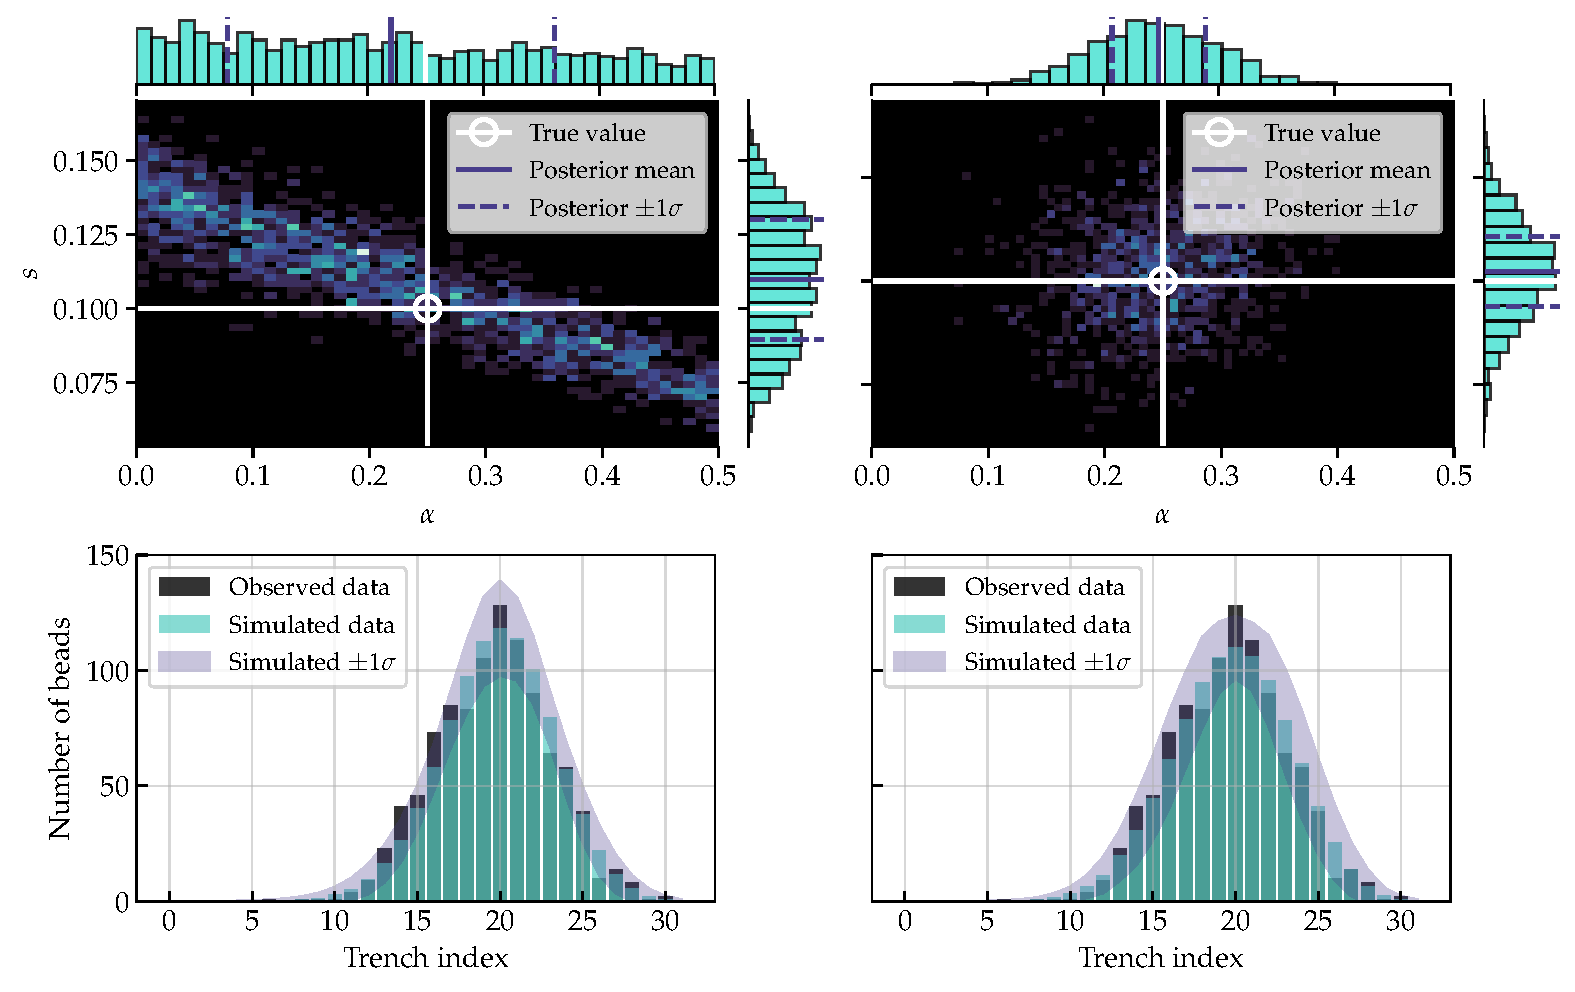
\includegraphics[width=0.99\textwidth]{figs/dalton_sim_comp.pdf}
    \vspace{-0.4cm}
    \caption{ABC results for acceptance rate $\approx 1\%$ using two different summary statistics: mean only (left) and mean, variance, skewness, kurtosis (right). Top panels show the joint posterior distribution of $\alpha$ and $s$. Bottom panels show the posterior predictive histograms compared to the observed data with $\pm 1\sigma$ uncertainty bands.}
    \label{fig:dalton_sim}
\end{figure}
\vspace{-0.2cm}
The left panel of Figure~\ref{fig:dalton_sim_NN} shows the corresponding results for the extended summary statistic ABC when NN-based proposals are used to generate a prior for the latent tilt $s$. The figure displays a very narrow distribution of $s$, centered about $s_\text{true}$, and a clearly more concentrated posterior for $\alpha$ around $\alpha_\text{true}$ than in Figure~\ref{fig:dalton_sim}. The middle panel shows the sampled bead distribution with one standard deviation compared to observed data. The sampled data produces a distribution closer to the observed data, and with a lower $\pm 1\sigma$ compared to the sampled distributions in Figure \ref{fig:dalton_sim}. The right panel shows the training and validation loss for the NN used to propose the prior of $s$. The NN converges rapidly, with both training and validation loss decreasing sharply during the first few iterations and then approaching a low, stable value close to zero. % The two loss curves stay very close to each other, with the validation being slightly lower throughout the iterations.
\begin{figure}[H]
    \centering
    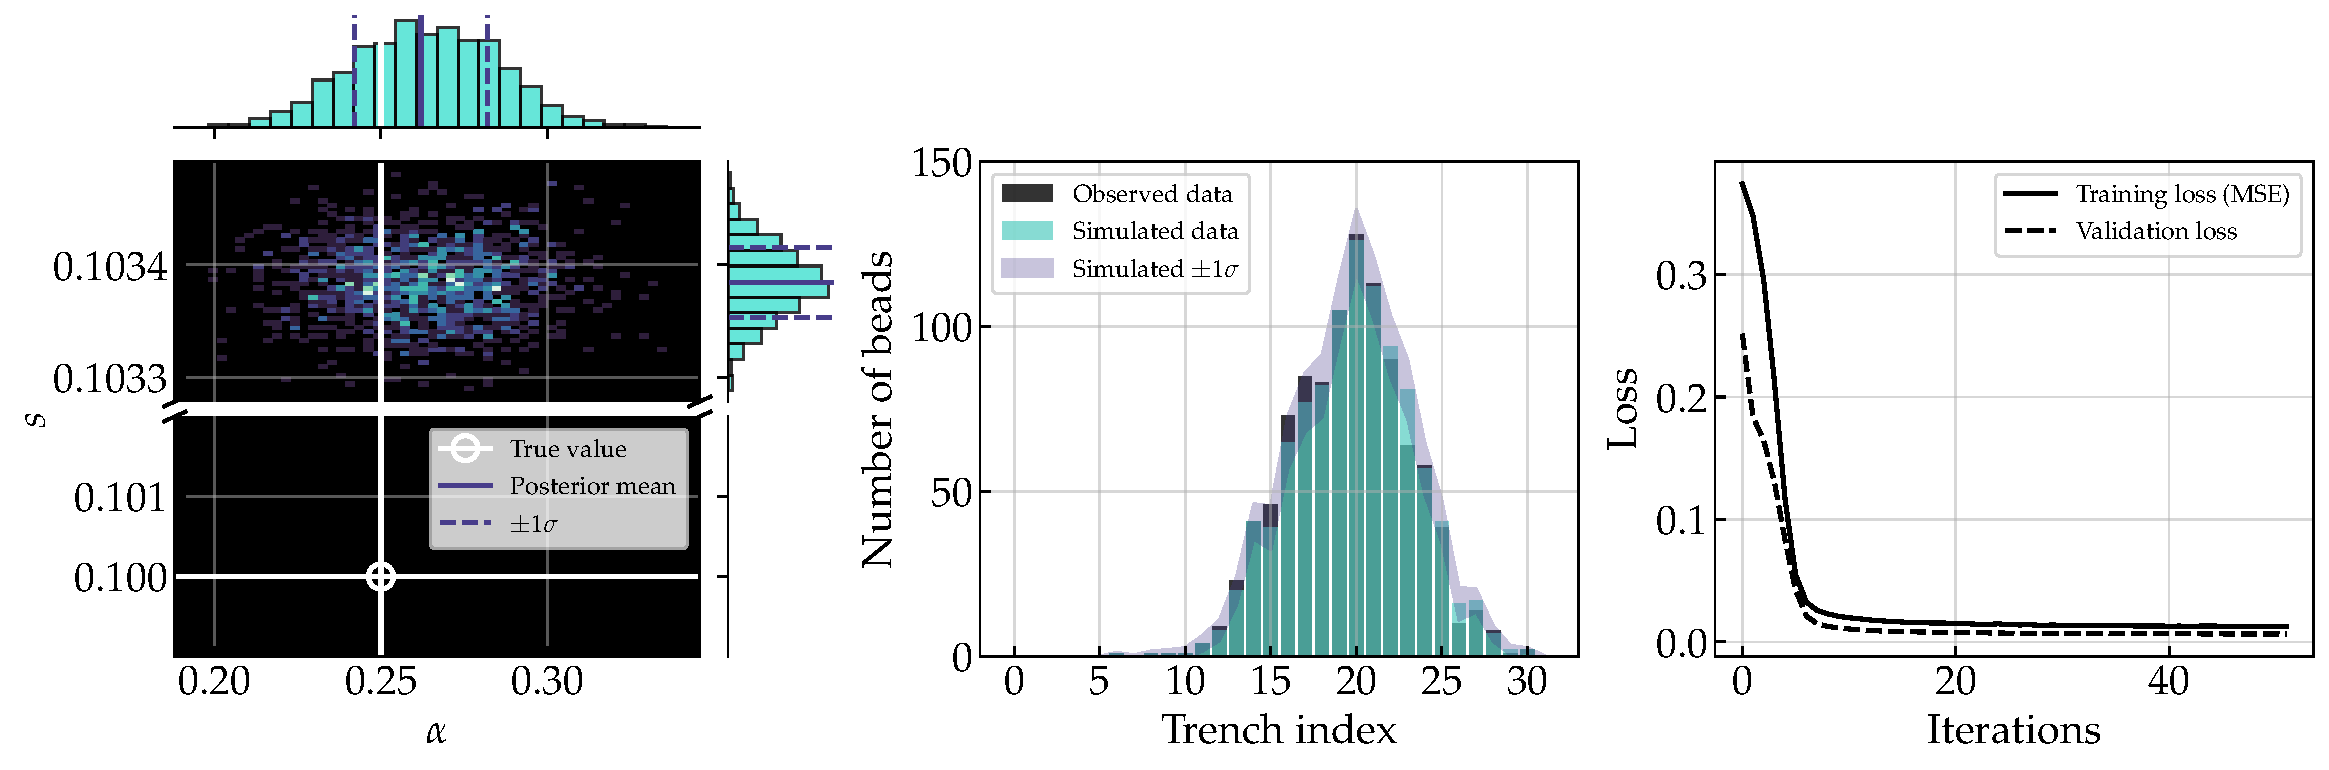
\includegraphics[width=0.99\textwidth, trim={0.2cm, 0.2cm, 0.2cm, 0.2cm}, clip]{figs/dalton_ABC_NN_summary_comparison_combined.pdf}
    \vspace{-0.3cm}
    \caption{The joint posterior distributions of $\alpha$ and $s$ (left) and posterior predictive histograms (middle) for ABC with NN-based proposals for $s$, four-moment summary statistics, and $\approx 1\%$ acceptance rate. The right plot shows the training and validation loss curves for the NN used to propose $s$.}
    \label{fig:dalton_sim_NN}
\end{figure}

Figure~\ref{fig:trans} shows the results from the iterative posterior transformations to infer the most likely $\alpha$. The left panel shows the mean estimate of $\alpha$ for each posterior transformation, a $\pm 1\sigma_\alpha$ band, together with the values of $\sigma_\alpha$ on the second $y$-axis. The estimate converges to $\alpha \approx 0.330$, and the uncertainty decreases as the number of transformations increases, stabilizing very close to zero. The right panel displays the corresponding posterior means of $s$ for each transformation. As expected, these values vary randomly, since the tilt changes uncontrollably between experiments.
\begin{figure}[H]
    \centering
    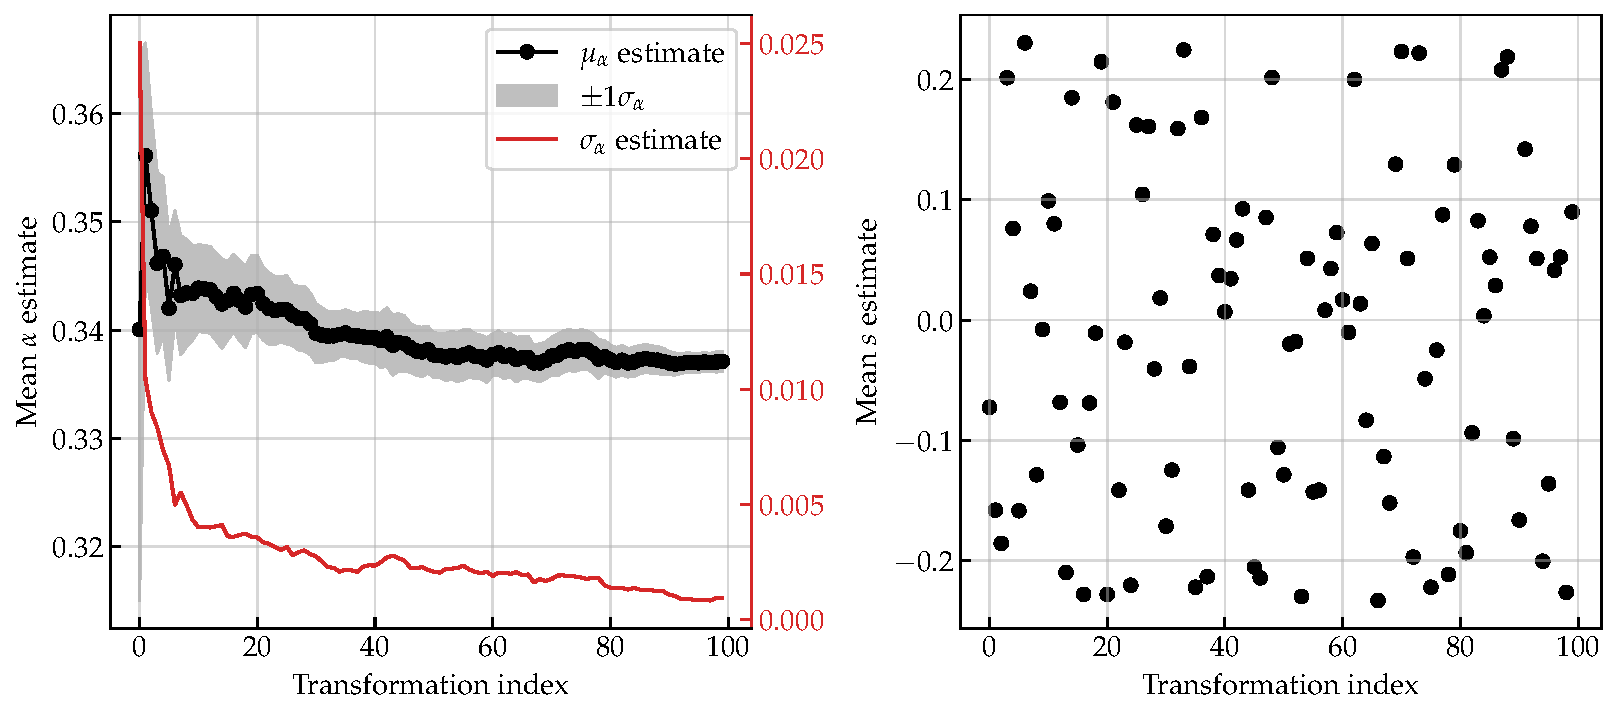
\includegraphics[width=0.99\textwidth]{figs/dalton_ABC_transformation_estimates.pdf}
    \vspace{-0.4cm}
    \caption{The sample mean estimates of $\alpha$ (left) and $s$ (right) for each posterior transformation, together with a $\pm 1\sigma_\alpha$ band and the values of $\sigma_\alpha$ on the left panel.}
    \label{fig:trans}
\end{figure}
\vspace{-0.8cm}
\section{Discussion}
The synthetic tests give a first check that the ABC method behaves in the expected way. For both choices of summary statistics, the posterior distributions for $\alpha$ and $s$ cover the true values $(\alpha_\text{true}, s_\text{true}) = (0.25, 0.10)$. This indicates that the method can locate the correct region in parameter space. At the same time, Table~\ref{tab:summary_stats_comparison} shows that the quality of the inference depends strongly on both the acceptance rate and the information included in the summary.

A lower acceptance rate generally gives tighter posteriors, which is reflected in smaller posterior standard deviations. In addition, the estimates improve when the posterior means move closer to the true parameter pair $(0.25, 0.10)$. The effect is most important for $\alpha$. When only the mean is used, $\mu_{\alpha}$ remains below $0.25$ and $\sigma_{\alpha}$ stays comparatively large across acceptance rates. This suggests that the mean alone does not contain enough information to constrain $\alpha$. This is consistent with the shape of the posterior when using mean only. It appears stretched along a direction where $\alpha$ and $s$ trade off against each other, since many combinations of $\alpha$ and $s$ can reproduce a similar overall shift of the bead distribution.

When the four moment summary statistics are used, the picture changes. Including variance, skewness, and kurtosis adds distribution information about width and shape. This reduces the degeneracy between $\alpha$ and $s$ and the posterior becomes more concentrated around $(0.25, 0.10)$. The improvement is strongest at low acceptance, where $\mu_{\alpha}$ move closest to the true values while the posterior standard deviations decrease ($\mu_{\alpha}$ is insubstantially affected). The distribution for $\alpha$ also becomes closer to normal rather than being nearly flat, which supports the conclusion that the four moment summary statistics are better suited for identifying $\alpha$. For $s$, the mean already helps somewhat, but the most consistent overall performance is obtained when the four moment summary statistics are combined with low acceptance.

% The synthetic tests give a first check that the ABC method behaves in a reasonable way. In both choices of summary statistics the posterior distributions for $\alpha$ and $s$ include the true values $(\alpha^*, s^*)$, so the basic setup is able to find the right region in parameter space. The stretched shape of the posterior when only the mean is used as summary shows a clear dependence on $s$ and at the same time a large uncertainty in $\alpha$. Both parameters influence how far the bead distribution is shifted, so many combinations of $\alpha$ and $s$ can match the same center of mass.

% Adding variance, skewness and kurtosis changes this picture. These moments contain information about the width and asymmetry of the distribution, which are affected in different ways by $\alpha$ and $s$. With the four moment summary, the posterior becomes much more concentrated around $(\alpha^*, s^*)$, and the distribution of $\alpha$ looks close to a normal distribution instead of being almost flat. This indicates that the more detailed summary captures the dependence on both parameters and is better suited for the inference problem.

Introducing the NN to construct proposals for $s$ improves the precision further. The posterior for $s$ becomes very narrow and is centered close to $s_\text{true}$, and the posterior for $\alpha$ also tightens around $\alpha_\text{true}$. The predictive histograms follow the synthetic data closely and the uncertainty band shrinks. This suggests that the approach can recover $(\alpha_\text{true}, s_\text{true})$ very accurately when the NN and the more intricate summary statistics are used together. At the same time, the NN can introduce a small bias. In the present example, the posterior for $s$ does not completely cover $s_\text{true}$, as seen in Figure~\ref{fig:dalton_sim_NN}. A likely explanation is that the NN prediction produces a slight over-estimate of $s$. In that case, most simulations are drawn in a region that is shifted compared to the true tilt. Since no explicit correction for the difference between the original prior and the NN based proposal is made, this shift will be reflected in the posterior for $s$. The estimate of $\alpha$ is still very close to $\alpha_\text{true}$, but the small bias in $s$ could potentially affect the accuracy of the $\alpha$ estimate as well. This highlights the importance of having a well-trained NN that can predict $s$ accurately.

At the same time, the NN can introduce a small bias. In the present example, the posterior for $s$ does not completely cover $s^*$. A likely explanation is that the NN prediction is a slight over-estimate of $s$. In that case, most simulations are drawn in a region that is shifted compared to the true tilt. Since no explicit correction for the difference between the original prior and the NN based proposal is made, this shift will be reflected in the posterior for $s$. The estimate of $\alpha$ is still very close to $\alpha^*$ here, but in principle a stronger NN bias could lead to biased posteriors in some parts of parameter space.
For the given Galton board data $y_\text{obs}$, the chained ABC runs are mainly interesting for what they say about the method as a whole. The simulation construction combines information from many data sets under the assumption that $\alpha$ is the same in all experiments and that $s$ changes from one experiment to the next. With this setup, it is expected that the chain of posterior transformations moves the posterior for $\alpha$ toward a relatively narrow distribution and that later transformations only change it slightly. 

This is indeed what is observed in Figure~\ref{fig:trans}, where the mean estimate of $\alpha$ converges after about 40 transformations and the uncertainty $\sigma_\alpha$ decreases steadily. After 100 transformations, the final estimate is $\alpha \approx 0.330 \pm 5.469 \cdot 10^{-6}$. The remaining uncertainty does not mean that the method has failed to converge, but instead reflects the limits of the information in the data and the approximations that are made. Each experiment contains a finite number of beads, so there is a natural limit to how well $\alpha$ can be determined, since different $\alpha$ values can produce similar distributions due to random fluctuations. The tilt $s$ is never observed directly and is only handled through the NN based proposals, so some degeneracy between $\alpha$ and $s$ remains. On top of this, there is the ABC approximation itself and the choice to represent the posterior for $\alpha$ as a normal distribution at each step. The fact that the inferred $s$ values fluctuate between data sets fits well with the idea of a rocking board and supports the modeling assumption that $\alpha$ is shared while $s$ varies from experiment to experiment.

Regarding improvements to the proposed method, the possibilities are essentially endless. We have already explored and outlined how the addition of more summary statistics improves the inference results. Of course, other summary statistics could be explored as well, for example percentiles of the distribution or other moments. On the other hand, using more summary statistics increases the dimensionality of the distance metric, which can increase the computational cost. Thus, it is important to find a balance between informativeness and efficiency. Another avenue for improvement is the NN architecture and training process. In this project, we used a simple feed-forward NN with one hidden layer and ReLU activation. However, more advanced architectures, such as convolutional NNs or recurrent NNs, could potentially capture more complex relationships between the data and the parameters. Another option is to implement an adaptive kernel size $h$ that decreases over time, allowing for a more refined approximation of the posterior as the ABC procedure progresses. Additionally, instead of proposing $s$ and $\alpha$ separately, a joint proposal distribution could be learned using the NN, which might capture correlations between the two parameters more effectively. Overall, there is much room for further exploration and improvement in the methods demonstrated in this project.

\printbibliography

\end{document}